\chapter{Bitmap Graphics}

The \jr\ supports three different graphics modes: bitmaps, sprites, and tiles. Bitmaps provide for a static, screen-sized image. Tiles provide a screen-sized image that is composed of a static set of tiles, which may be rearranged and scrolled around the screen. Sprites provide smaller, movable images. All three grapihcs engines use the same general principle of how pixel colors are determined, those pixels are just arranged in different ways.

At the core of an image on the \jr\ is the pixel data. This pixel data is a sequence of bytes somewhere in the first 256 KB of RAM, which is interpreted by TinyVicky as being a rectangular block of pixels, the size and layout of which varies. Each pixel is represented by a single byte, which takes on a value from 0 to 255. This number serves as an index into a graphics color lookup table (CLUT). The CLUT contains 256 4-byte entries, which specify the RGB components of the color (plus one currently unused byte). As an example, let's say that a given pixel is the byte 0x05. When drawing that pixel on the screen, TinyVicky will look up the color in the sixth entry of the CLUT for that image. If the value in that entry is $({\rm red}, {\rm green}, {\rm blue}) = (0, 0, 128)$, then the pixel will be drawn in a medium blue (see figure~\ref{fig:bitmap_colors}).

\begin{figure}[h]
    \begin{center}
        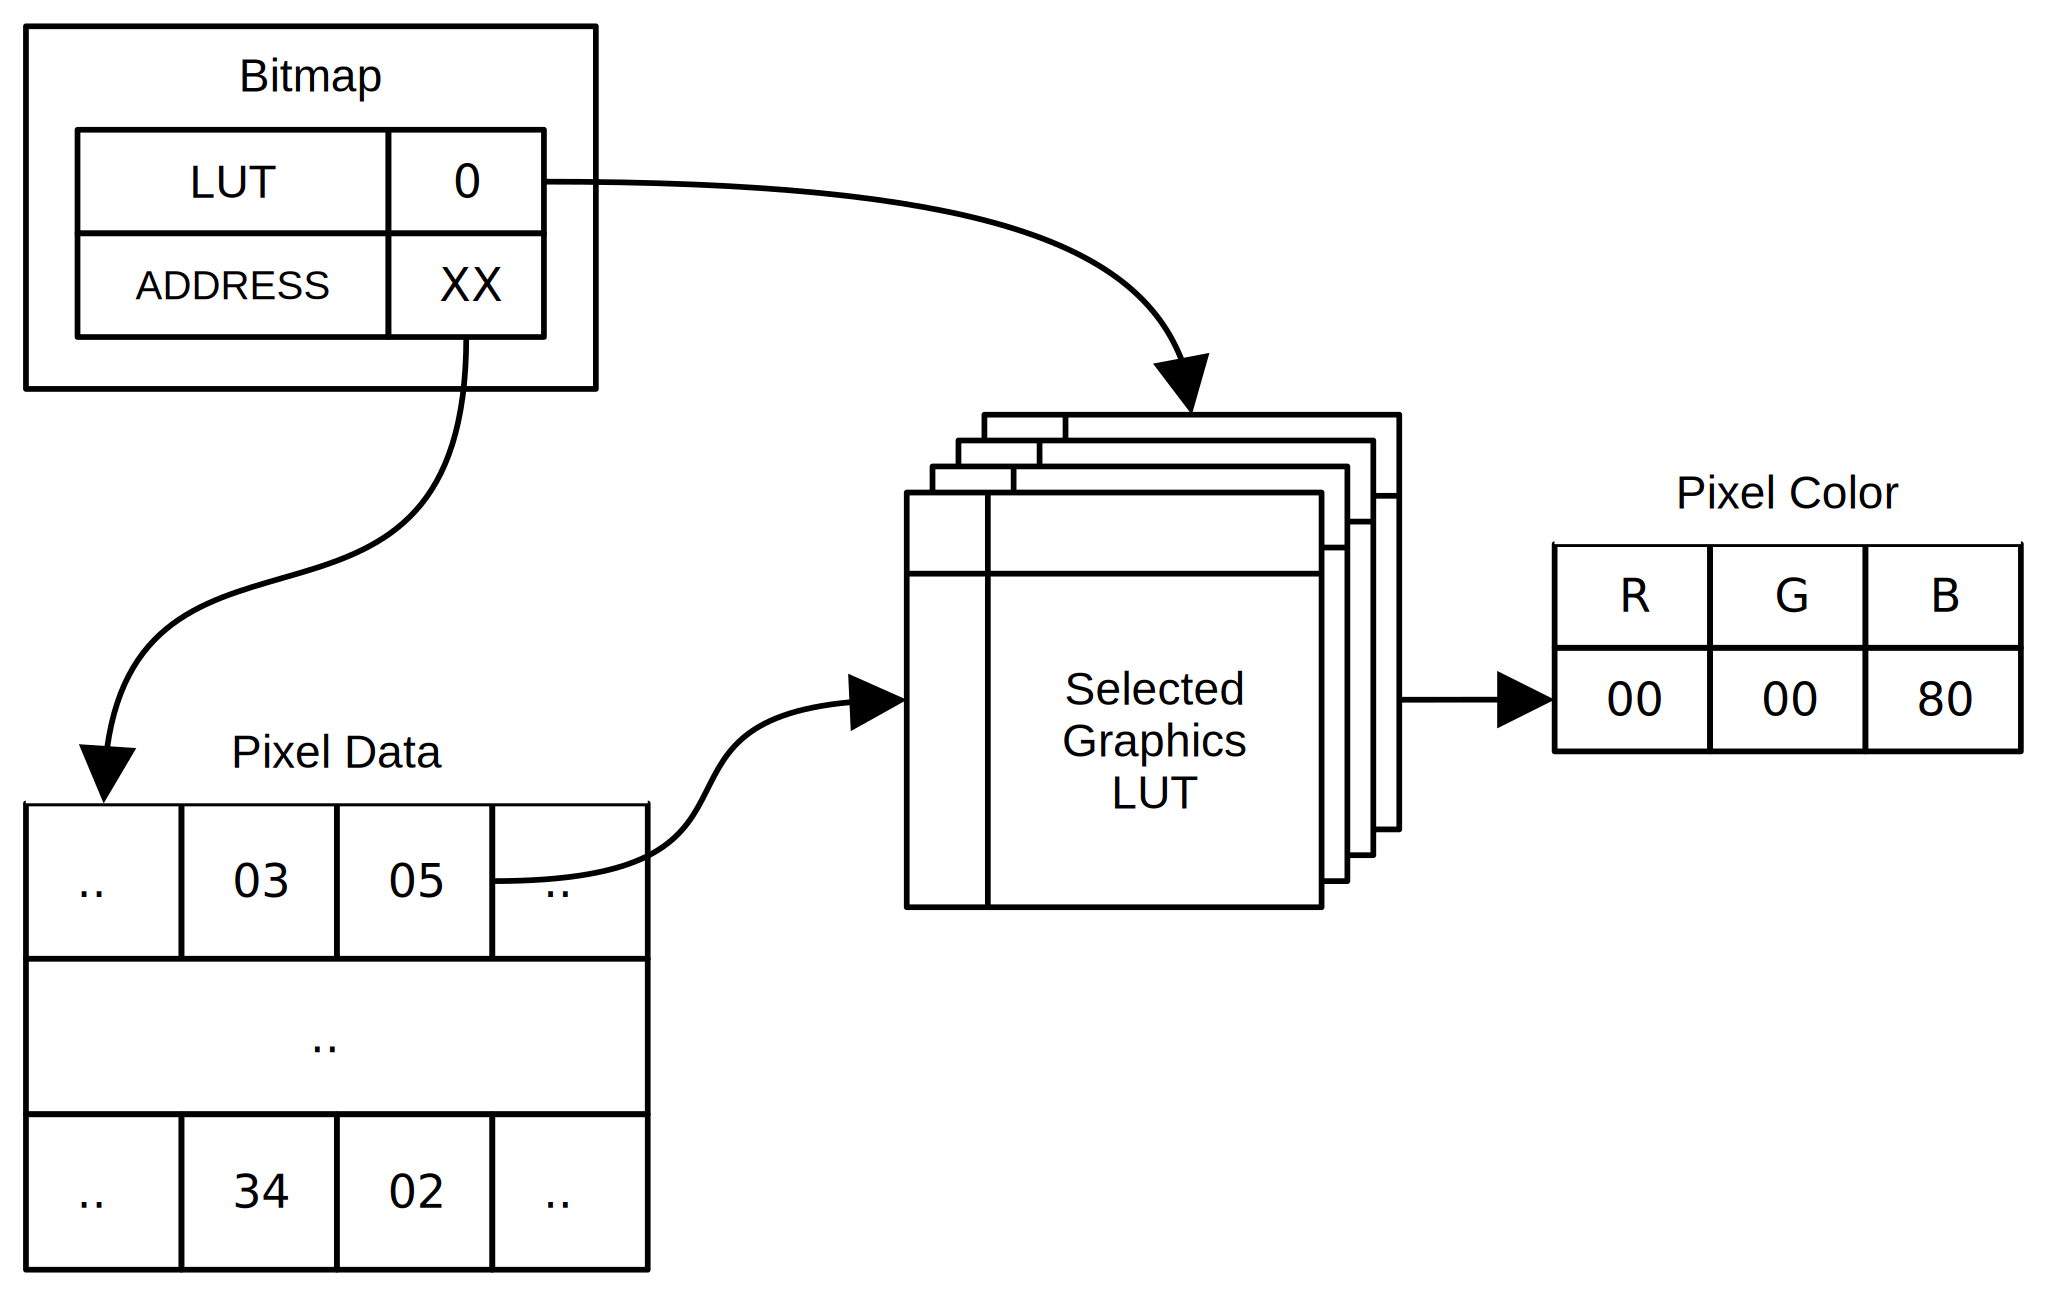
\includegraphics{images/bitmaps.pdf}
    \end{center}
    \caption{Bitmap Data to Pixels}
    \label{fig:bitmap_colors}
\end{figure}

Color 0 is special. It is used as the transparent or background color. The color of a pixel in that color will be the color of whatever is behind it or of the background color if there is nothing else behind it. TinyVicky provides seven layers of graphics. There are four layers that sprites can be assigned to, and there are three layers that can be assigned either a bitmap or a tile map. These layers are interleaved, so sprite layer 0 is the front most layer, followed by layer 0 for bitmaps and tile maps, followed by sprite layer 1, and so on (see figure~\ref{fig:layers}).

\begin{figure}[h]
    \begin{center}
        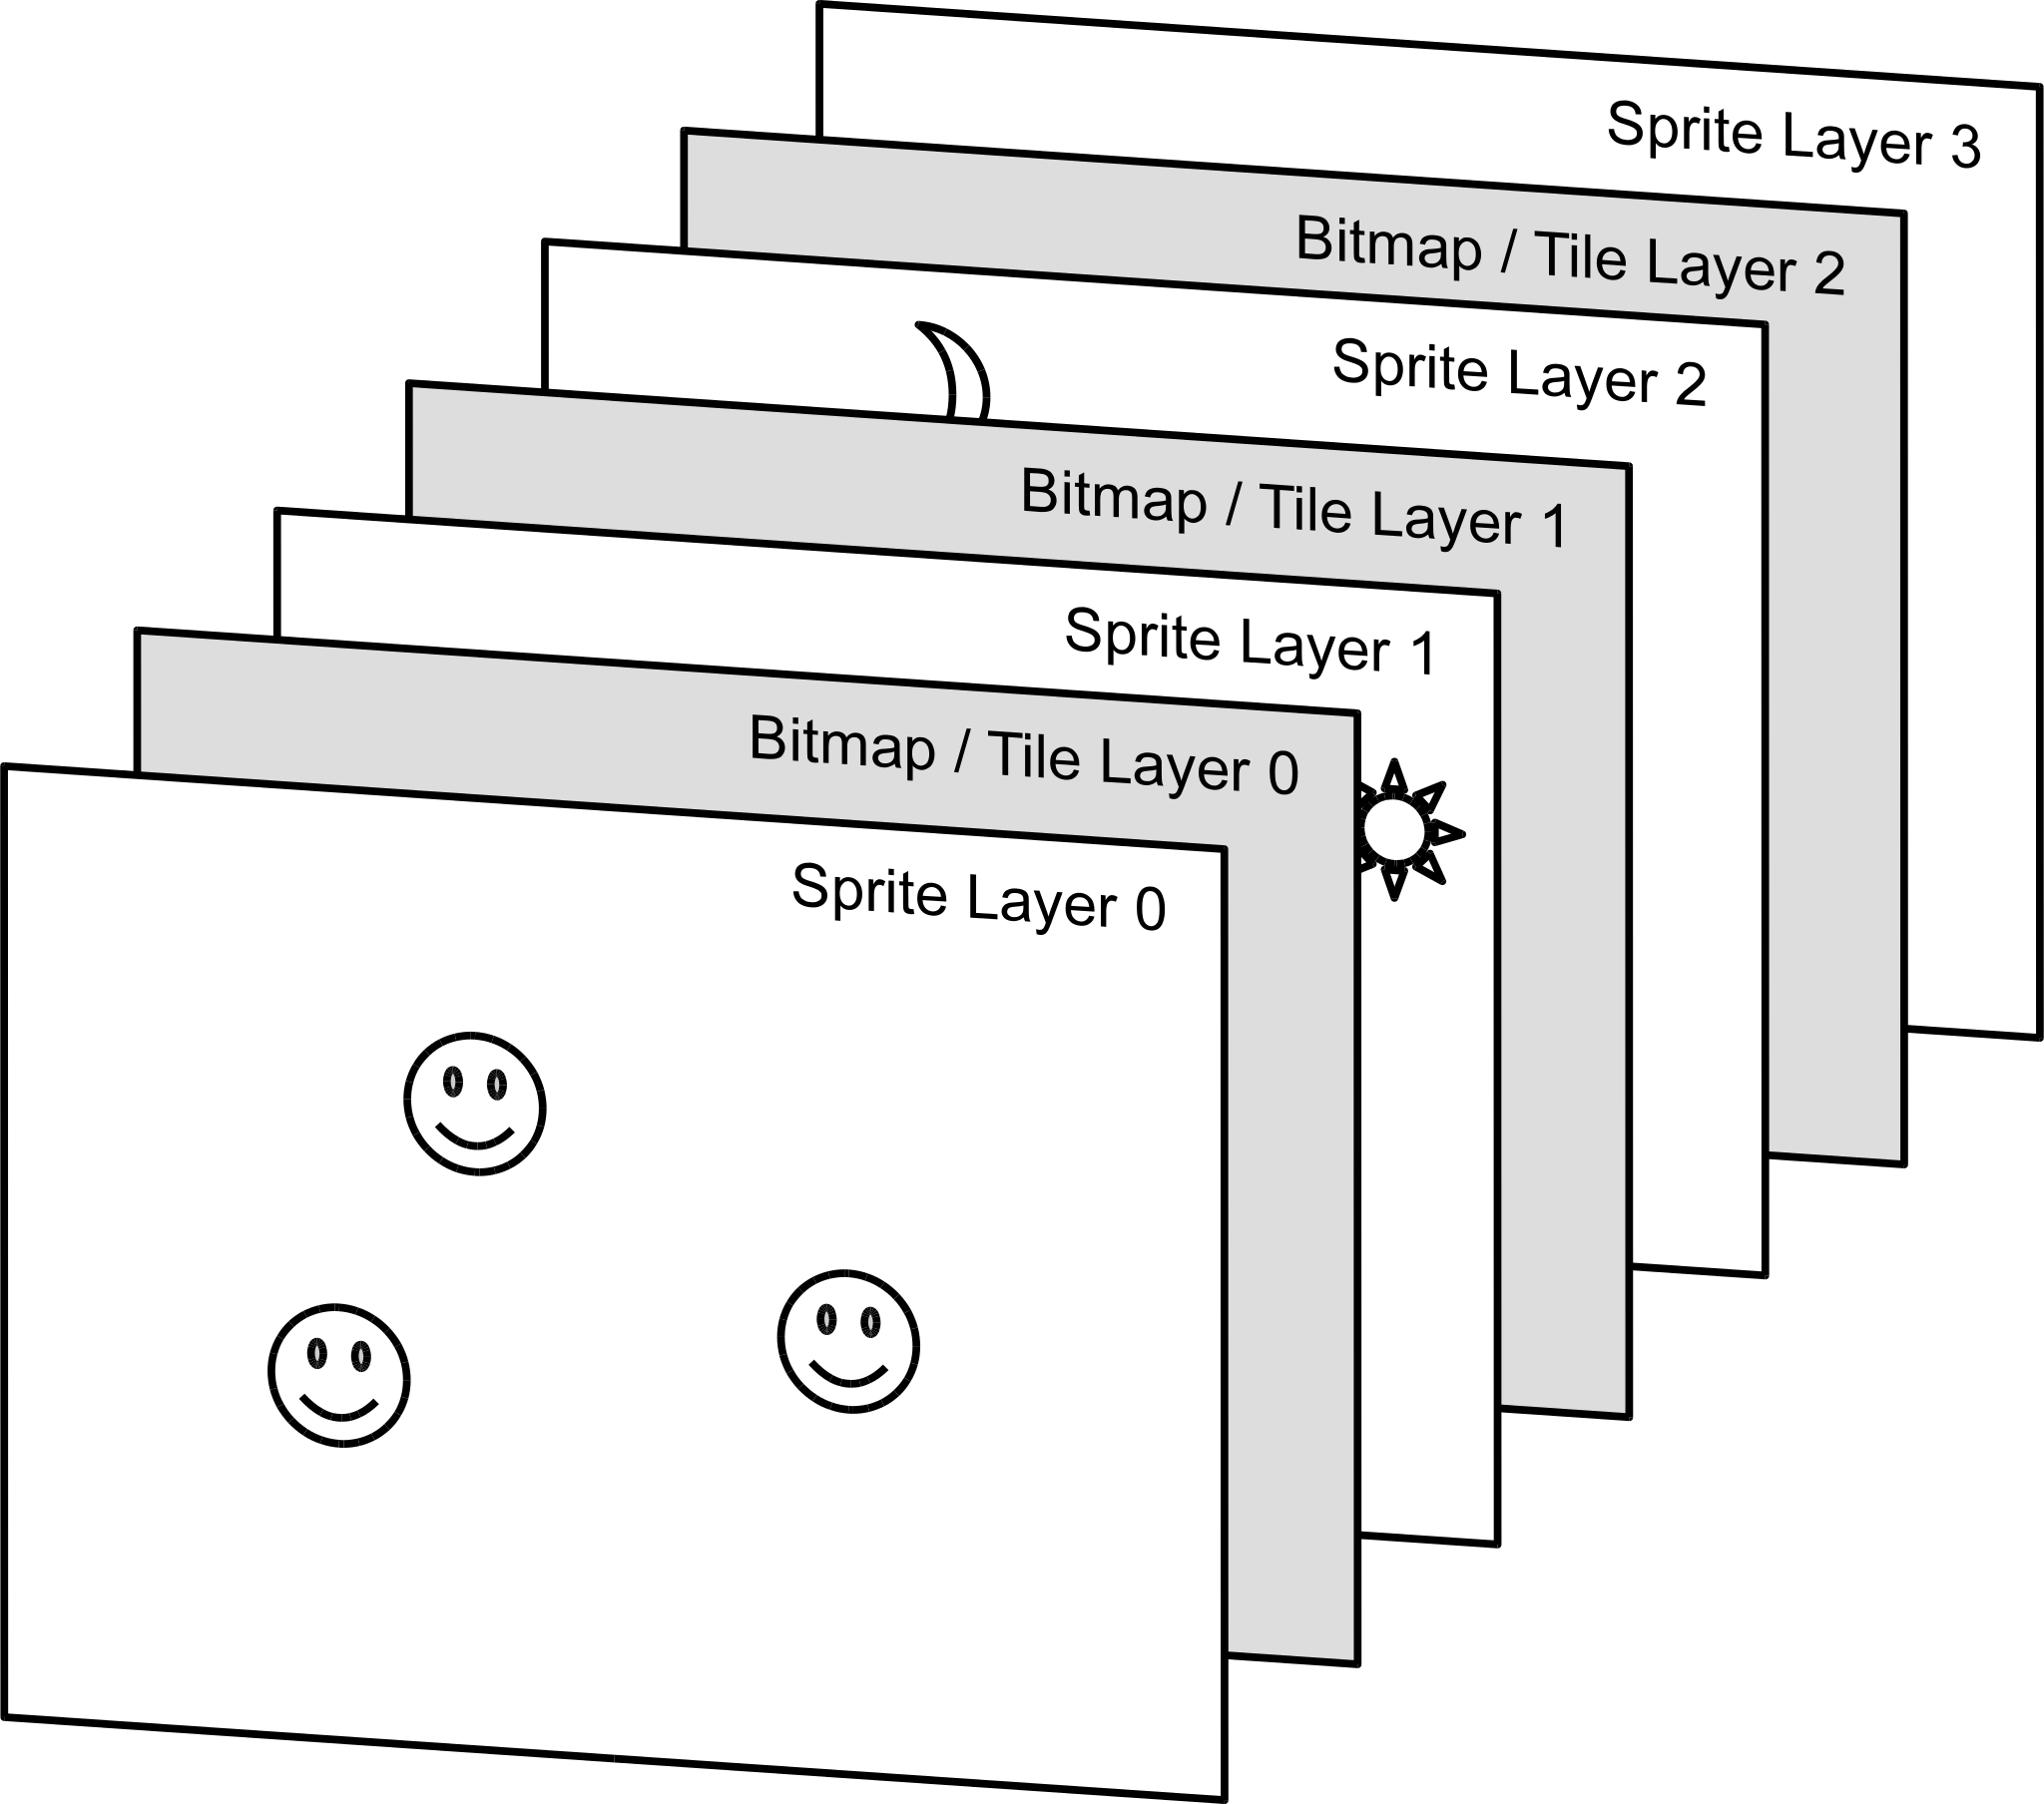
\includegraphics{images/Layers.pdf}
    \end{center}
    \caption{TinyVicky Graphic Layers}
    \label{fig:layers}
\end{figure}

\begin{table}[h]
    \begin{center}
        \begin{tabular}{|c|c|c|c|c|c|c|c|c|} \hline
            Address & 7 & 6 & 5 & 4 & 3 & 2 & 1 & 0 \\ \hline\hline
            \verb+0xD002+ & --- & \multicolumn{3}{|c|}{LAYER1} & --- & \multicolumn{3}{|c|}{LAYER0} \\\hline
            \verb+0xD003+ & \multicolumn{5}{|c|}{---} & \multicolumn{3}{|c|}{LAYER2} \\\hline
        \end{tabular}
    \end{center}
    \caption{Bitmap and Tilemap Layer Registers}
    \label{tab:bm_tm_layers}
\end{table}

The three fields LAYER0, LAYER1, and LAYER2 in the layer registers are three bit values, which indicate which graphical element to assign to that layer (see table~\ref{tab:bm_tm_lay_mapping}).

\begin{table}[h]
    \begin{center}
        \begin{tabular}{|c|c|c||l|} \hline
            0 & 0 & 0 & Bitmap 0 \\\hline
            0 & 0 & 1 & Bitmap 1 \\\hline
            0 & 1 & 0 & Tile Map 0 \\\hline
            0 & 1 & 1 & Tile Map 1 \\\hline
            1 & 0 & 0 & Tile Map 3 \\\hline
        \end{tabular}
    \end{center}
    \caption{Layer Mapping}
    \label{tab:bm_tm_lay_mapping}
\end{table}

\section{Bitmaps}

TinyVicky allows for two full screen bitmaps to be displayed at once. These bitmaps are either $320 \times 200$ or $320 \times 240$, depending on the value of the CLK\_70 bit of the master control register. A bitmap's pixel data contains either 64,000 bytes, or 76,800 bytes of data. In both cases, the pixel data is arranged from left to right and top to bottom. The first 320 bytes are the pixels of the first line (with the first pixel being the left-most). The second 320 bytes are the second line, and so on. Additionally, the bitmaps can independently use any of the four graphics CLUTs to specify the colors for those indexes. TinyVicky provides registers for each bitmap set the CLUT and the address of the bitmap:

\begin{table}[h]
    \begin{center}
        \begin{tabular}{|c|c|c|c|c|c|c|c|c|c|} \hline
            Address & Bitmap & 7 & 6 & 5 & 4 & 3 & 2 & 1 & 0 \\ \hline\hline
            \verb+0xD100+ & \multirow{4}{*}{0} & \multicolumn{5}{|c|}{---} & \multicolumn{2}{|c|}{CLUT} & ENABLE \\\cline{1-1}\cline{3-10}
            \verb+0xD101+ & & AD7 & AD6 & AD5 & AD4 & AD3 & AD2 & AD1 & AD0 \\\cline{1-1}\cline{3-10}
            \verb+0xD102+ & & AD15 & AD14 & AD13 & AD12 & AD11 & AD10 & AD9 & AD8 \\\cline{1-1}\cline{3-10}
            \verb+0xD103+ & & \multicolumn{6}{|c|}{---} & AD17 & AD16 \\ \hline
            \verb+0xD108+ & \multirow{4}{*}{1} & \multicolumn{5}{|c|}{---} & \multicolumn{2}{|c|}{CLUT} & ENABLE \\\cline{1-1}\cline{3-10}
            \verb+0xD109+ & & AD7 & AD6 & AD5 & AD4 & AD3 & AD2 & AD1 & AD0 \\\cline{1-1}\cline{3-10}
            \verb+0xD10A+ & & AD15 & AD14 & AD13 & AD12 & AD11 & AD10 & AD9 & AD8 \\\cline{1-1}\cline{3-10}
            \verb+0xD10B+ & & \multicolumn{6}{|c|}{---} & AD17 & AD16 \\ \hline
        \end{tabular}
    \end{center}
    \caption{Bitmap Registers}
    \label{tab:bm_registers}
\end{table}

\begin{description}
    \item[ENABLE] if set and both graphics and bitmaps are enabled in the Vicky Master Control Register (see table~\ref{tab:vky_master_ctrl_reg}), then this bitmap will be displayed.

    \item[CLUT] sets the graphics color lookup table to be used for this bitmap

    \item[AD] give the address of the first byte of the pixel data within the 256 KB system RAM. Note that this address is relative to the system bus of 20 bits and is not based on the CPU's addressing.
\end{description}
